\documentclass[10pt, twocolumn]{article}
\usepackage{amssymb}
\usepackage{graphicx}
\usepackage{simpleConference}
\usepackage{subcaption}
\usepackage{svg}
\usepackage{times}
\usepackage{url,hyperref}

\begin{document}

\title{Moving Object Detection from a Moving Camera}

\author{Masahiro Ogawa\\
  \\
  Yamashita An Lab,
  Department of Precision Engineering,
  University of Tokyo, Japan\\
  Mini thesis\\
  \today
  \\
  \\
  ogawa@robot.t.u-tokyo.ac.jp}

\maketitle
\thispagestyle{empty}

\begin{abstract}
 We develop the state of the art accuracy moving object detection from a moving camera.
 The basic idea of our algorithm is if the camera is moving straight forward, we extract moving object as strange flow considering the computed focus of expansion, otherwise we assume the camera is rotating and extract moving objects as undominant flow area. At the same time, to reduce false positives, we incorporate optical flow and semantic segmentation information (not yet implemented for this mini thesis).
 Our approach accomplish state of the art accuracy on our qualitative evaluation.
\end{abstract}



\section{Introduction}
Separating moving and static objects is very important for real environment applications.
Such applications include obstacle avoidance for autonomous vehicles, and scene understanding for assistant robots.

There are many researches about this topic.
The most frequently adopted approach would be optical flow orientation based approach.
However if the camera is going straightforward, the flow orientation will spread radially, and the flow orientation approach will fail.
To overcome this problem, we take Focus of Expansion (FoE) based approach.
By computing FoE and estimate the flow based on FoE, we successfully treat the problem.

\begin{figure}[t]
  \centering
  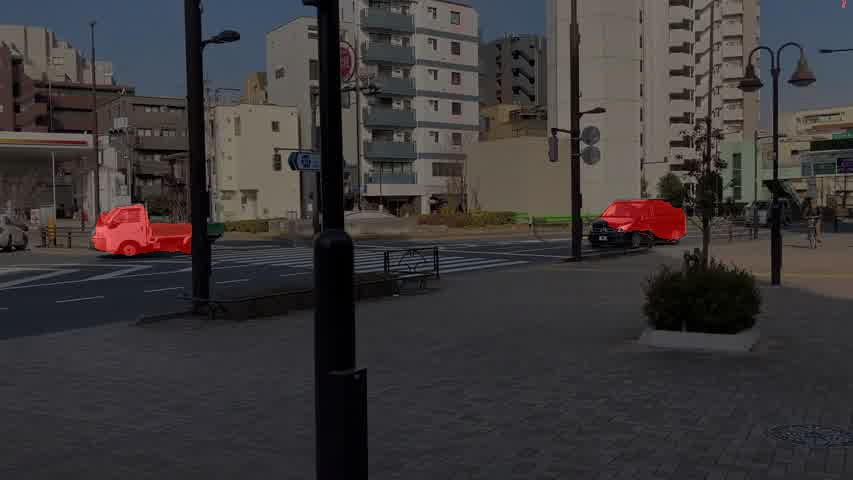
\includegraphics[width=8cm]{fig/exampleoutput.jpg}
  \caption{Example output of our moving object detection from a moving camera.}
  \label{fig:exampleoutput}
\end{figure}


\section{Rerated Work}
There have been several papers on moving object detection from a moving camera.
One of the famous review paper about moving object detection from a moving camera is Chapela et al's one \cite{chapel2020moving}.
They categorized moving object detection methods, but did not do quantitative evaluation nor create a ranking.
Another famous review paper is X.Zhao et al's one \cite{ZHAO202228}.
They categorized methods and provided rankings.
The highest-ranking method is Motion U-Net2 \cite{DBLP:conf/icpr/RahmonBSP20}.
They used gray scale monocular video as an input and combined three channels; gray scale image, background subtraction image, and flux mask.
However, this method only works for slightly moving cameras and cannot handle large camera motions.

On the other hand, the best method on paperswithcode web site of the category; "Semi-Supervised Video Object Segmentation on Davis (no YouTube-VOS training)" is "HMMN" \cite{DBLP:journals/corr/abs-2109-11404}.
However this method requires human inputs of target initial positions, which means this method is not moving object detection in our definition but is just a tracking algorithm.

In addition to search reviews, we also search state of the art approaches.

W.Zhang et al \cite{Zhang_Sun_Yu_2020} developed a optical flow orientation based approach.
They used the orientation of the optical flow between adjacent frames and calculates the background orientation field.
The motion saliency is obtained by the difference between the reconstructed background orientation and the region orientation.
Their results looks good, but they didn't provide the quantitative comparison between current state of the art methods.

Hu an Uchimura \cite{hu2000} developed Focus of Expansion (FoE) based approach to extract moving objects from a moving camera.
This method estimates the camera rotation and translation using pre-computed FoE.
Then, if the rotation compensated optical flow is not the one which expected for static objects, it will consider the pixel comes from moving objects.
However, this method assumes a fixed FoE because it assumes car mounted camera.
Therefore if the camera is handheld, as our assuming case, it will not work anymore.

One of the current state-of-the-art approach is Yang et al's deep adversarial network based approach \cite{yang_loquercio_2019}.
They used an adversarial network for optical flow information.
The generator tries to create a mask that is hard to estimate the inside mask flow, while the in-painter tries to estimate the flow inside the mask.
The loss is computed by the information reduction rate.
Although this method performed well on their evaluation data set, but had some issues when we tested on our data set.
There are some false positives in low-textured areas and large object motion regions, where is hard to estimate optical flow from surrounding flow.


\section{Proposed Method}
The concept of our method for detecting moving objects from a moving camera is 1. extract self motion using FoE, 2. combine optical flow and texture cues.
To detect moving objects, we found that estimating self camera motion at the same time is necessary.
\begin{figure}[ht]
  \centering
  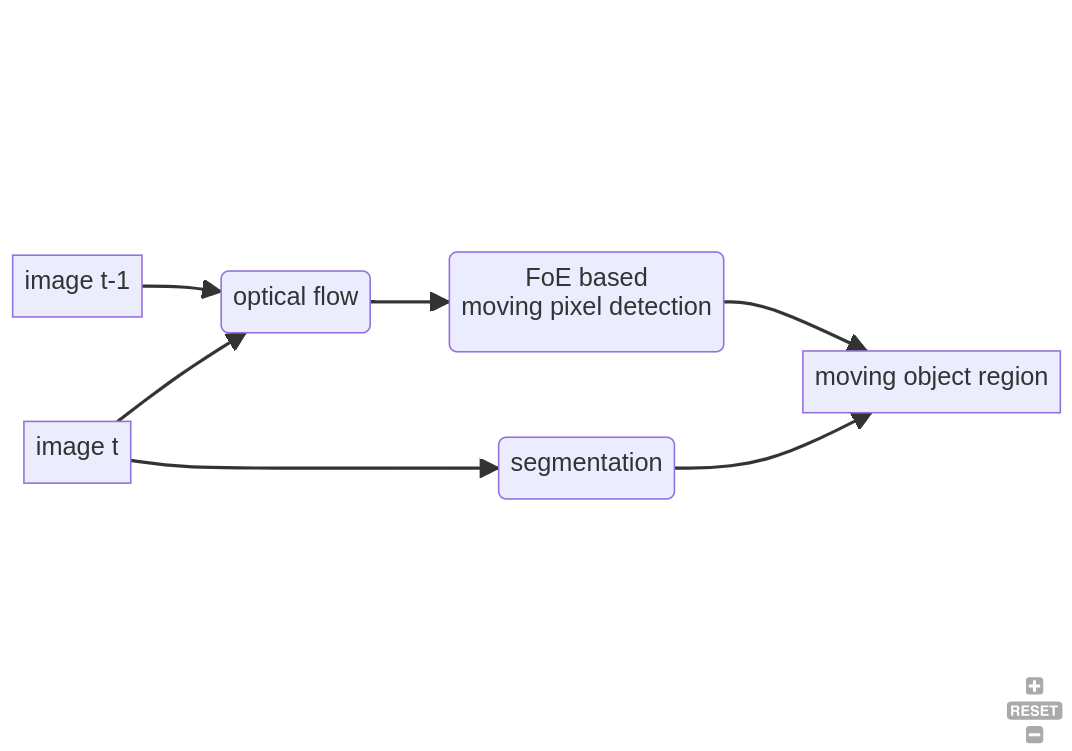
\includegraphics[width=8cm]{fig/wholeflow.png}
  \caption{Flow chart of proposed method.\\
    Rectangle box means an object and rounded box means a process.}
  \label{fig:wholeflow}
\end{figure}
The overall abstract procedure is in Figure \ref{fig:wholeflow}.

To compute optical flow, we adopt top ranked method in paperswithcode, which is named UniMatch\cite{xu2022unifying}.
This approach extracts features by CNN and match features by transformer.

After computing optical flow, we compute the FoE from the obtained flow using RANSAC.
\begin{figure}[ht]
  \centering
  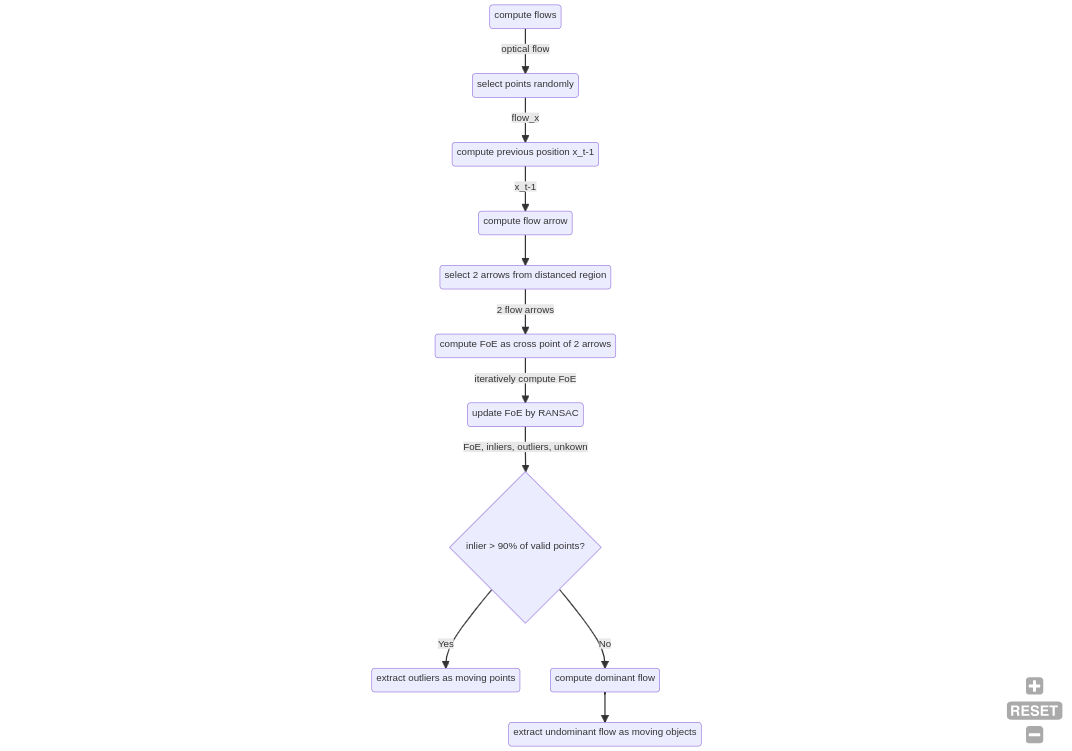
\includegraphics[width=8cm]{fig/foeflow.png}
  \caption{Detail flow chart of FoE based moving pixel detection}
  \label{fig:foeflow}
\end{figure}
The detail of ``FoE based moving object pixel'' in Figure \ref{fig:wholeflow} is in Figure \ref{fig:foeflow}.

Our approach does not consider refining the rotation effect for computing FoE as in \cite{hu2000}, because it cannot estimate both the FoE and rotation simultaneously.
Therefore if the inliers of FoE in RANSAC is not enough (this time, we set it as less than 90\%), we judge the camera is rotating.
If it is judged that the camera is rotating, we extract the different orientation flows as the moving pixels.
Otherwise, if the inlier is large enough, we trust the computed FoE and extract the pixels which does not follow the orientation computed from the FoE as moving object pixels.
Then, we combine the moving object pixels with segmentation information to extract the final moving object region.


\section{Evaluation}

\subsection{Qualitative Evaluation}
We used our own dataset to compare the results of our method with the state-of-the-art method ``contextual information separation \cite{yang_loquercio_2019}''.

\begin{figure}[ht]
  \centering
  \begin{minipage}{0.3\linewidth}
    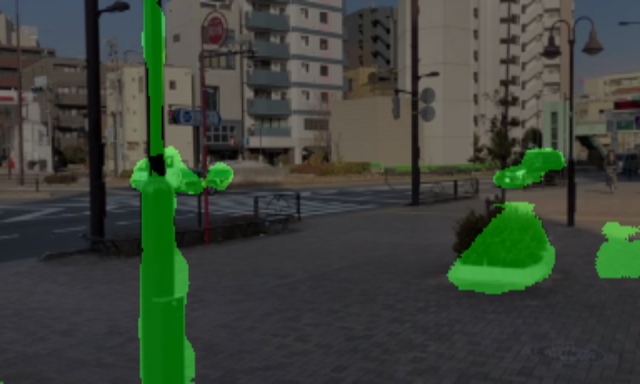
\includegraphics[width=\linewidth]{fig/contextual/frame_00000002.png}
    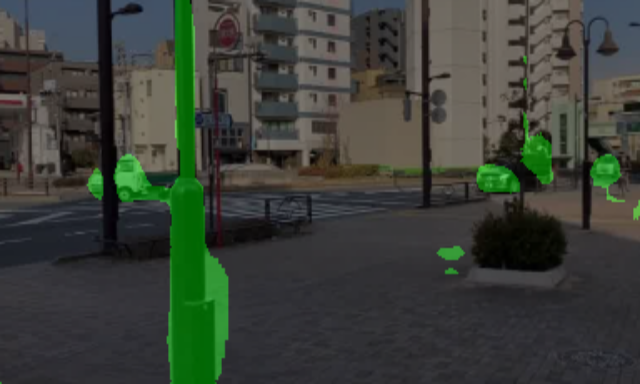
\includegraphics[width=\linewidth]{fig/contextual/frame_00000010.png}
    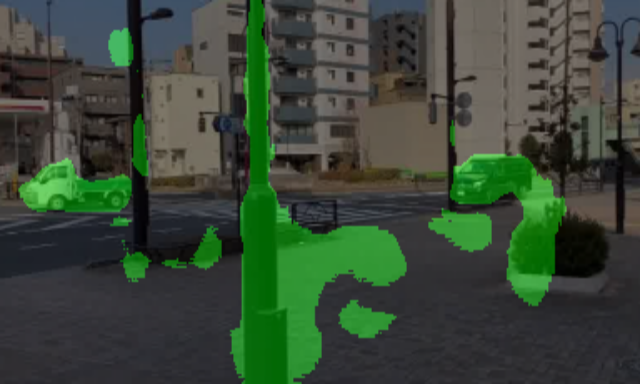
\includegraphics[width=\linewidth]{fig/contextual/frame_00000020.png}
    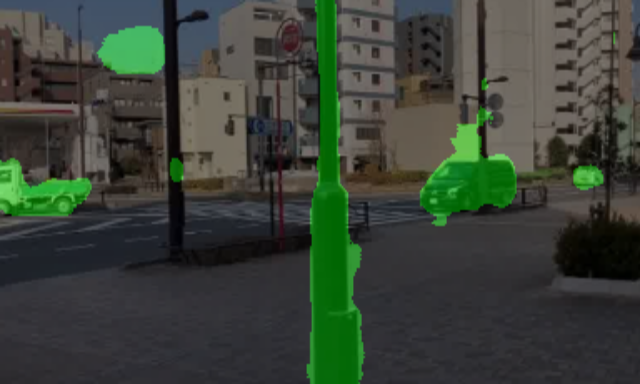
\includegraphics[width=\linewidth]{fig/contextual/frame_00000030.png}
    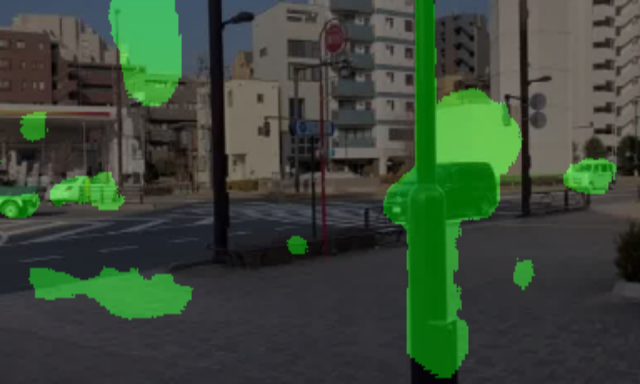
\includegraphics[width=\linewidth]{fig/contextual/frame_00000040.png}
    \caption*{Contextual information separation}
  \end{minipage}
  \hfil
  \begin{minipage}{0.3\linewidth}
    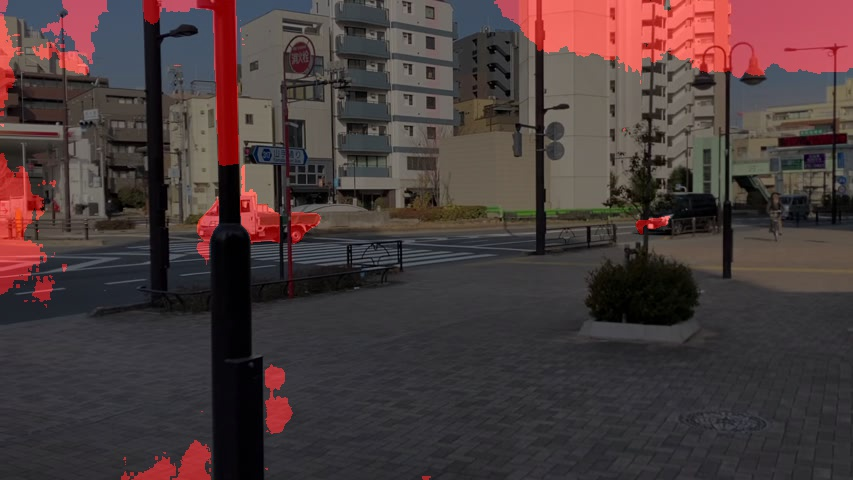
\includegraphics[width=\linewidth]{fig/proposed/00002.jpg}
    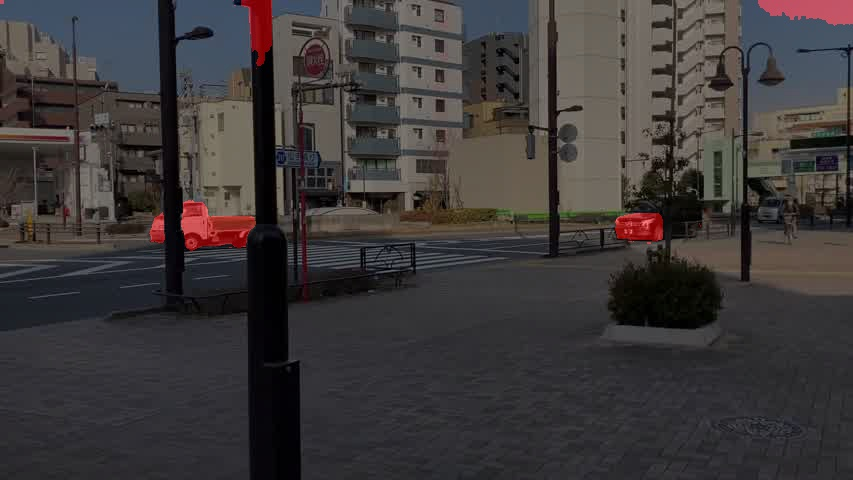
\includegraphics[width=\linewidth]{fig/proposed/00010.jpg}
    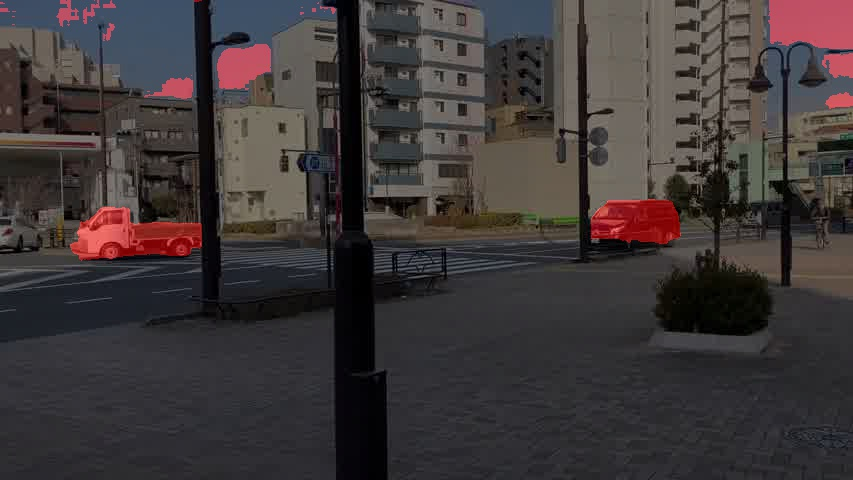
\includegraphics[width=\linewidth]{fig/proposed/00020.jpg}
    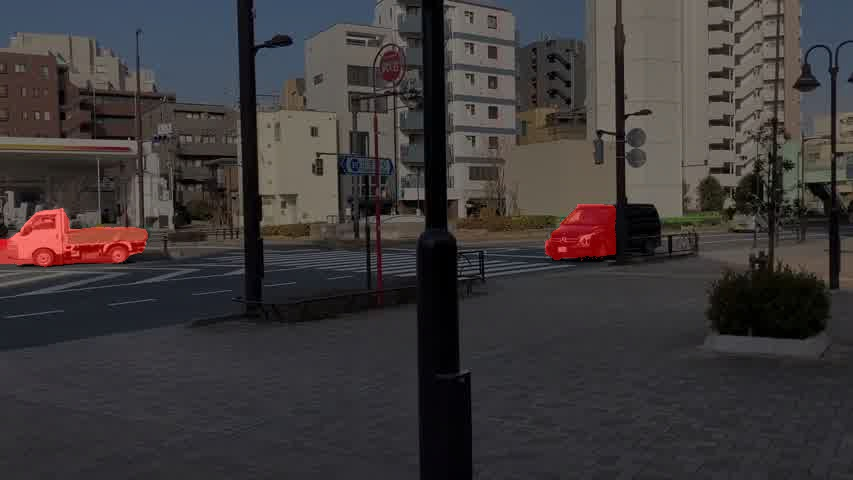
\includegraphics[width=\linewidth]{fig/proposed/00030.jpg}
    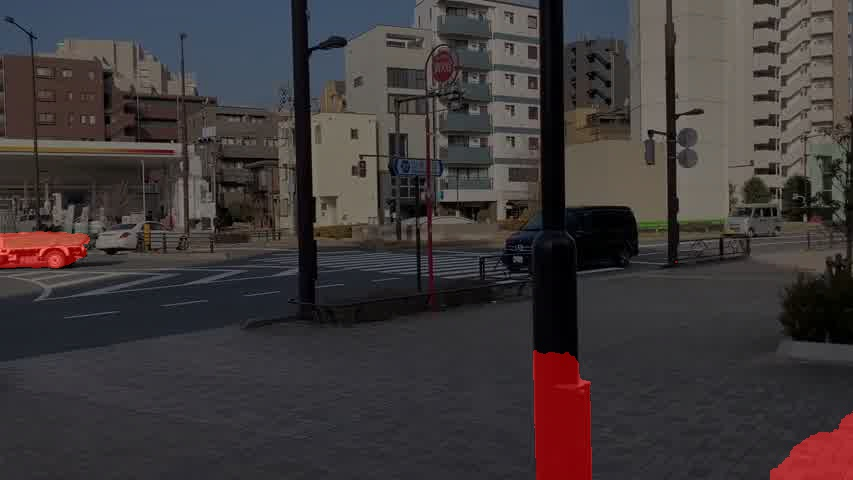
\includegraphics[width=\linewidth]{fig/proposed/00040.jpg}
    \caption*{Proposed method}
  \end{minipage}
  
  \caption{Qualitative comparison for the same scene between contextual information separation and proposed method.\\
  Proposed method can detect close poles as static object compared with contextual information separation method.}
  \label{fig:comparison}
\end{figure}

The result images is in Figure \ref{fig:comparison}.
Our approach successfully extracted moving object areas compared to the failure of Adversarial Network in large optical flow areas.


\subsection{Quantitative Evaluation}
For quantitative evaluation, we will use the Davis data set, which is commonly used for moving object detection.
However, we have not yet finished the implementation, so there are no quantitative evaluation results available at this time.


\section{Summary}
In this paper, we have presented a state-of-the-art accuracy method for extracting moving objects from a moving camera.
Our method combines flow and segmentation information to achieve better results compared to existing state-of-the-art methods.

\subsection{Future Work}
We will incorporate segmentation information to reduce false positives of moving objects.
We plan to estimate camera motion using deep neural network instead of using traditional methods.
And we also plan to utilize Nerf \cite{mildenhall2020nerf}, and Object scene representation to extract 3D representation and object information.


\bibliographystyle{abbrv}
\bibliography{4dreconstruction}

\end{document}
